% $Id: conclusion.tex 
% !TEX root = main.tex

%%
\section{Validation}
\label{sec:validation}

%%%%
\subsection{Evaluation scenarios}
To evaluate the effectiveness of \adaptiverl in adapting to changing goals and new acquired actions 
we use two different scenarios. First, we use the Gridworld benchmark as a proof of concept 
evaluation and running example of \adaptiverl. Second we use a traffic-signal control scenario to 
validate the adaptation of agents' behavior in real-world scenarios.

%%%%%%
\subsubsection{Gridworld}
The Gridworld scenario is defined as described in \fref{sec:motivation}. We execute the Gridworld 
agents for $1,500$ episodes with a maximum of 36 steps per episode (until the episode concludes). 
The agents are executed for $1,000$ independent runs, to assure significance of the presented 
results.

The Gridworld scenario is split into two independent adaptation cases. In the first case, the 
environment's goal changes every 300 episodes, which for the agent should have learned the optimal 
policy. On every 300th episode, we change the goal to the diagonally opposite corner (\eg bottom-right 
corner on the first change). The goal is changed a total of five times throughout the $1,500$ episodes. 
After the goal change, the agent should detect the concept drift and converge to an optimal policy for 
the new goal state.

In the second case, we modified the set of actions the agent can take in episode 300. The action 
acquired by the agent is the ability to jump over walls. After detecting the change, the agent should 
incorporate the new action into the optimal policy, leading to episodes executing less steps. 

%%%%%%
\subsubsection{Traffic-signal control}
Intelligent traffic management is a canonical application of self-adaptive 
systems~\cite{HENRICHS2022106940}, and recent meta-\ac{RL} work has shown benefits when 
reward functions change with traffic saturation~\cite{meta-rl-traffic}. Here, we model two crossing 
lanes (C1 vertical, C2 horizontal) with Poisson arrivals and dynamically switch congestion levels 
(changing $\lambda$ parameter) to induce concept drift. 

In this scenario, the changes to the environment goals and agent actions take place simultaneously. 
The agent is given a new set of actions following a concept drift detected in a new reward function. 
This enables the agent to efficiently learn how to utilize the new actions and optimize traffic flow by 
adapting its policy to varying congestion levels. The agent acquires new capabilities without forgetting 
previously learned behavior, maintaining adaptability to changing environmental conditions.

We implement a custom \texttt{TrafficEnv} (extending OpenAI's Gym library~\cite{gymlib}). The system 
state $(c_1,c_2)$ represents the number of queued vehicles on lanes C1 and C2 respectively, where 
state values are bounded in the interval $[0,\mathit{max\_state}]$. At each time step the agent selects 
one of three signal phases (actions): $\{(5,2),\;(2,5),\;(3,3)\}$, indicating service capacities (percentage 
of the lane cleared per step) for C1 and C2, respectively. During each step, service is applied to C1, 
new vehicles arrive to C2 (a Poisson distribution with rate $\lambda_{2}$), then service is applied to 
C2, followed by arrival of new vehicles to C1 (a Poisson distribution with rate $\lambda_{1}$). Any 
unused service capacity incurs a penalty:
\[
\mathrm{penalty} \;=\; 3\times(\text{waste}_{C1} + \text{waste}_{C2})\,,
\]
discouraging over-serving lanes when queues are small.

The \emph{dynamic reward} combines congestion cost and service penalty, defined as 
$r - \mathrm{penalty}$, where:
\[
r = 
\begin{cases}
-(2c_1 + c_2)\quad &\text{if }c_1>7 \;\wedge\;c_1>c_2,\\
-(c_1 + 2c_2)\quad &\text{if }c_2>7 \;\wedge\;c_2>c_1,\\
-(c_1 + c_2)\quad &\text{otherwise}
\end{cases}
\]
The agents  execute for a total of $10,000$ episodes with 30 steps per episode. We induce two 
goal changes triggering a concept drift by changing arrival rate ($\lambda_1$ and $\lambda_2$ for 
the Poisson distributions) of vehicles: at episode $3,000$ we update the rates 
($\lambda_1, \lambda_2$) from $(4,2)\;\to\;(5,7)$, and at episode $8,000$ we update the rates from $(5,7)\;\to\;(3,1)$.


Note that when a drift is detected, agents acquires two new signal phases (\ie actions):
$(7,3)$ and $(3,7)$, allowing for finer control under high congestion. Old actions are never removed.

%%%
\subsection{Experimental setting}
All experiments are run on an Intel Core i5 with 64GB RAM. The experiments use version 3.12 of Python with the Gym library (0.26.2). 

For the evaluation in both application domains we compare the standard Q-learning algorithm (used as a baseline) and \adaptiverl.
\begin{itemize}
  \item \emph{Standard Q-learning} agents are defined with a fixed $\alpha=0.1$, and $\varepsilon$ decayed exponentially to $0.01$ from $0.9$.
  \item \adaptiverl agents use the PH-test to detect drifts in episode-rewards, resets $\varepsilon\!=\!1$ upon detection, and adaptively adjusts $\alpha$ based on the TD-error (\cf. \fref{sec:implementation}).  
\end{itemize}

%%%%
\subsection{Evaluation results}

%%%%%%
\subsubsection{Gridworld}

When comparing the results between \adaptiverl and Q-learning, we observe \adaptiverl consistently 
outperforms the base line in adapting to changing goals and acquiring new policies without forgetting 
previously learned knowledge. As shown in \fref{fig:q-value-comp}, after $1,500$ episodes, \adaptiverl 
maintains high Q-values for all previous goal configurations, whereas traditional Q-learning must 
overwrite its Q-values each time the goal relocates. Notably, \adaptiverl preserves prior knowledge by 
promoting exploration for a sufficient period after each detected drift and by scaling updates according 
to the TD-error magnitude. This approach not only prevents catastrophic forgetting but also enables 
the agent to handle both contradictory and non-contradictory overlapping subtasks---such as when 
goals are randomly sampled in nearby regions rather than at the exact same cell.\footnote{Animated simulations of these and other scenarios are available at: \url{https://anonymous.4open.science/r/morphin_rl/simulations/memory_stm_v4_exp.mp4}}

\adaptiverl introduces a modest overhead due to the detection of concept drift and adaptive updates. 
Nonetheless, the run-time efficiency the agents is actually lower. Using our experimental setting 
$1,000$ runs take approximately 5 minutes for \adaptiverl, while it takes around 8 minutes to 
complete all runs with the baseline Q-learning implementation. This efficiency gain results directly 
from the reduced number of steps needed to reach the goal after each drift. Specifically, \adaptiverl 
converges in significantly fewer steps than the standard agent --requiring about $1.9\times$ fewer 
iterations after the first conceptual drift and $1.7\times$ fewer over the full $1,500$ episodes; which 
highlights the practical advantages of our adaptive mechanisms in dynamic environments.

\fref{fig:q-value-comp} shows the state coverage and accumulated rewards for each of the Gridworld 
states after the $1,500$ episodes. The figure confirms (similar to the Figures \ref{fig:alpha} and 
\ref{fig:dynamic-eps}) that,= the agent is able to detect concept drift and learned to behave in the light 
of new environment conditions. In the heatmap, lighter colors represent a higher reward, showing how 
the lower right part of the grid has been explored successfully. Moreover, with or experiment design 
confirms the benefits of not forgetting, as after the second goal change, the visited states continue to 
have the same information as initially discovered (in proportion to the grid). At the end, the agent is 
more motivated to go towards the new goal, as that part of the environment has already been 
explored with good rewards around the new goal.
 
\begin{figure*}[hptb]
    \centering
    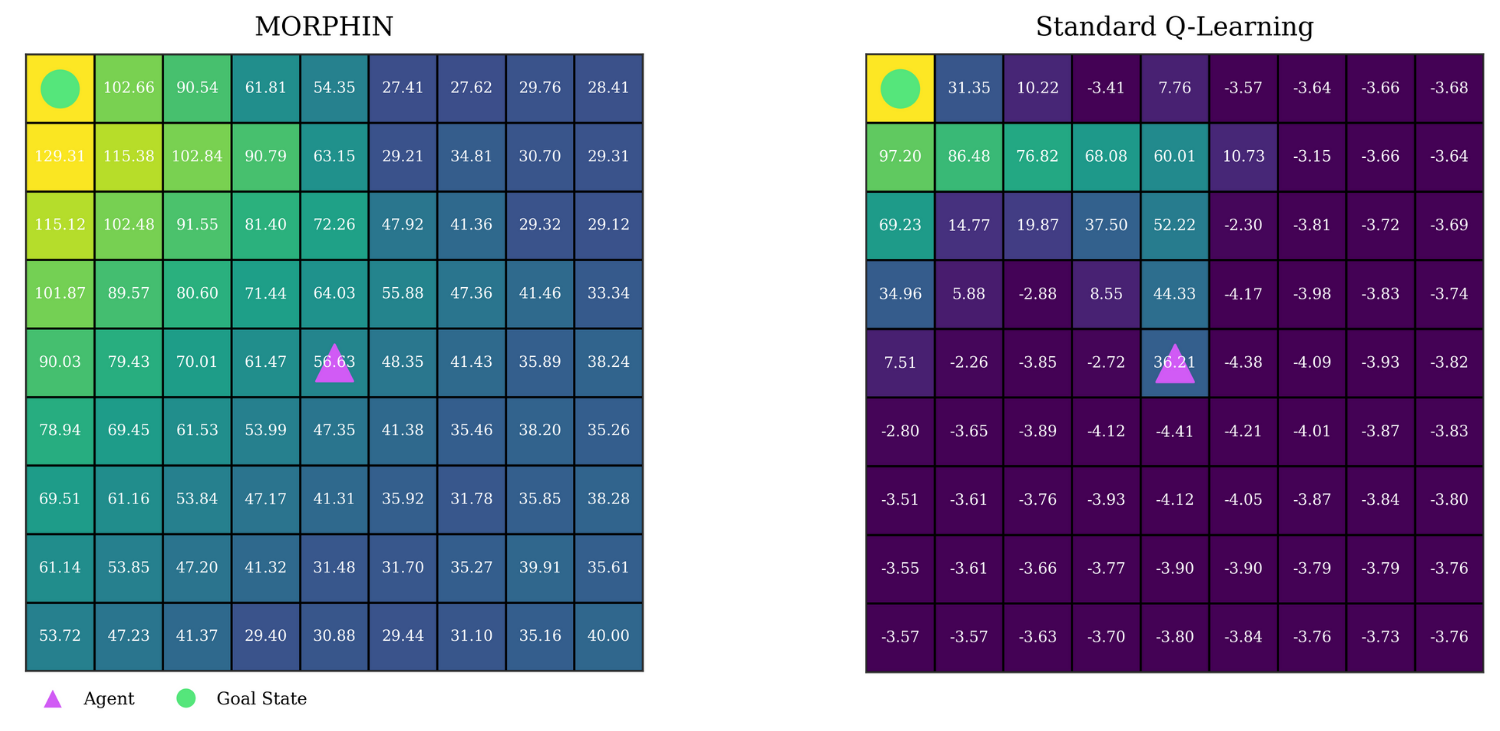
\includegraphics[width=0.9\textwidth]{figures/q_map_comp}
    \caption{Comparison of Q-value heatmaps after 1,500 episodes in a Non-Stationary Reward Environment: (left) \adaptiverl preserves high Q-values across alternating goal configurations; (right) Standard Q-learning must overwrite past knowledge to learn each new goal.}
    \label{fig:q-value-comp}
\end{figure*}

In the second case, when a new action is introduced, the \adaptiverl agent incorporates the new 
action as part of the optimal policy, reducing the actions taken from 14 to 4, by jumping over walls and 
other states. \fref{fig:q-value-comp2} shows the Q-value heatmaps after 400 episodes (300 episodes 
until the new action is introduced, and 100 episodes to find  the new policy including the acquired 
action). Upon introduction of the new action, \adaptiverl increases exploration and effectively learns 
to adjust its policy, leveraging the extended action set. In contrast, the baseline Q-learning agent only 
manages to apply the jump capability in previously unexplored states, as it has a higher chance of 
being used in such states than in states is a set policy. This results in a suboptimal policy after (taking 
14 steps to reach the goal) as the action space changes. 

\begin{figure*}[hptb]
    \centering
    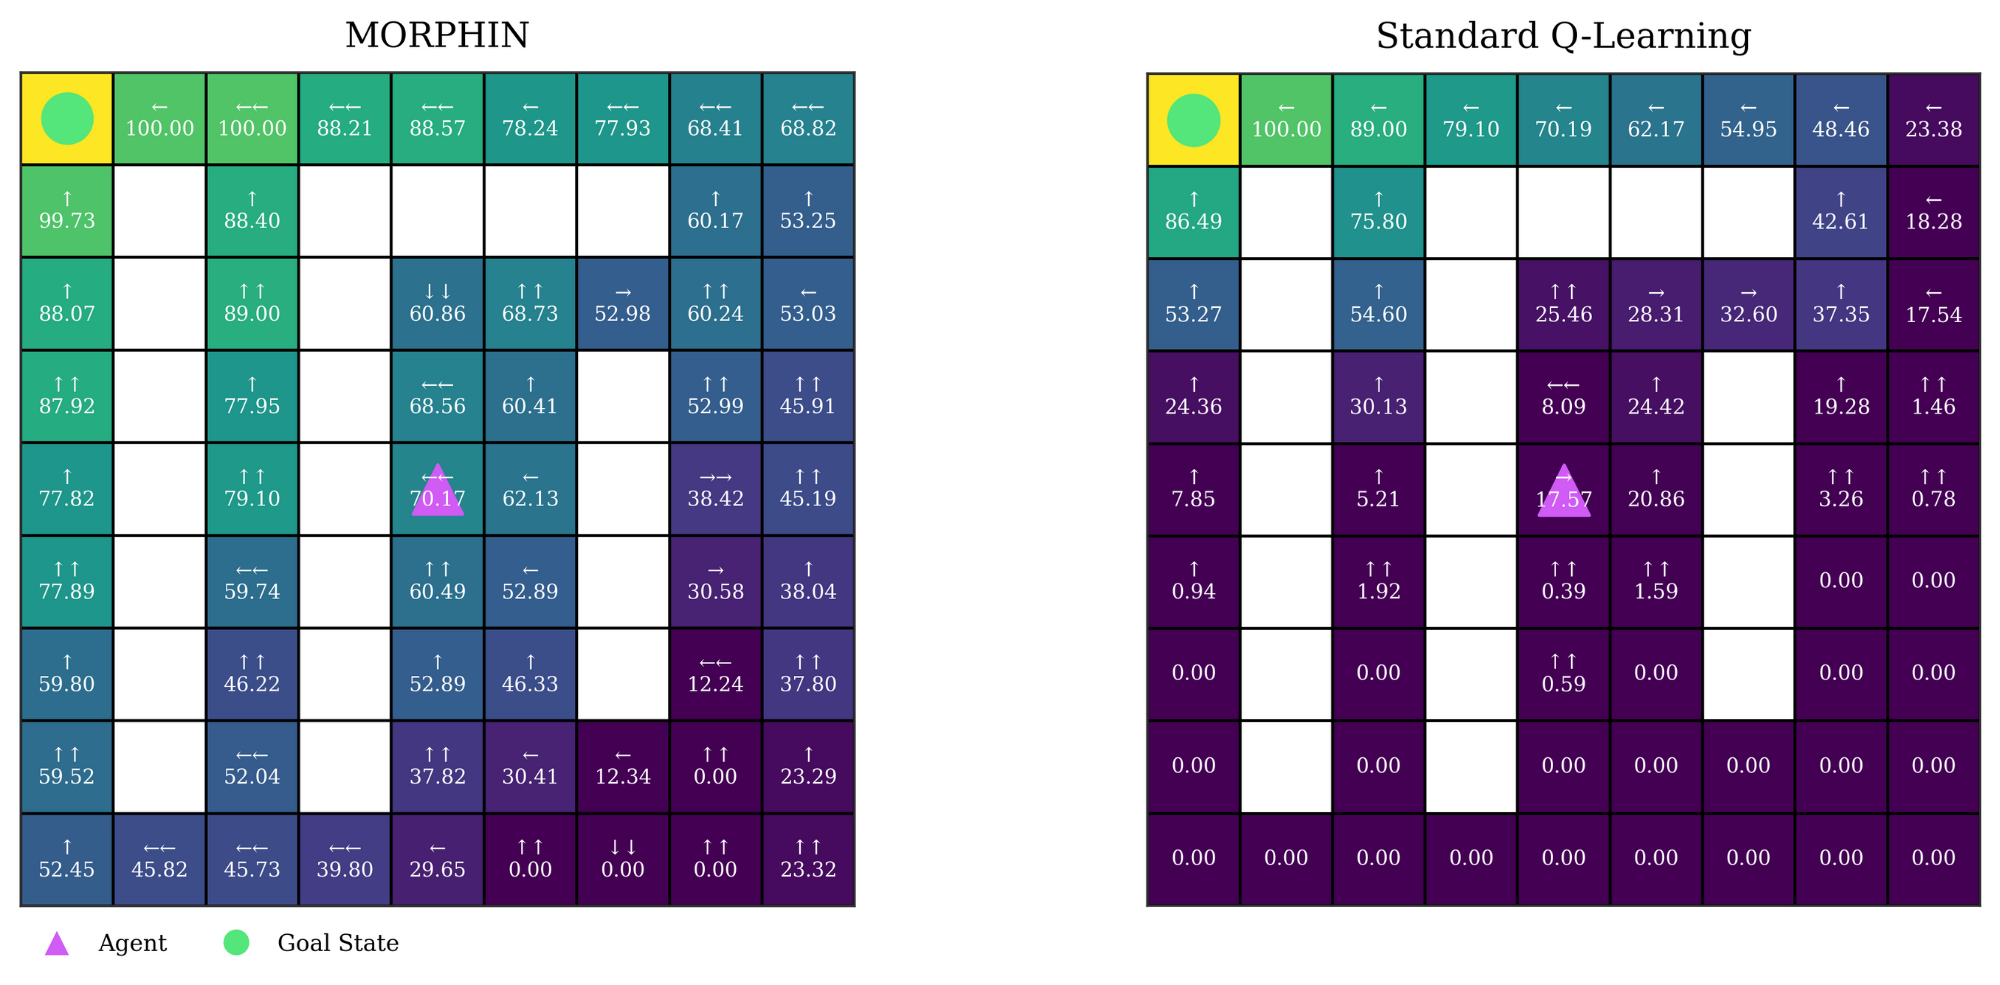
\includegraphics[width=0.9\textwidth]{figures/q_map_comp2}
    \caption{Comparison of Q-value heatmaps after 400 episodes with a mutable action space: (left) \adaptiverl effectively learns to use the extended set of actions, achieving an optimal policy for this configuration; (right) Standard Q-learning remains in a suboptimal policy for the new action space. Double arrows indicate the new actions available to the agent (jumping).}
    \label{fig:q-value-comp2}
\end{figure*}

This demonstrates how the adaptive mechanisms in \adaptiverl enable effective learning of new 
actions and adaptation to an expanded action space, while the standard Q-learning agent fails to do 
so.

%%%%%%
\subsubsection{Traffic-signal control}

We now focus on the results of using \adaptiverl in the traffic-signal control scenario under 
non-stationary congestion.  

\fref{fig:traffic-learning-curve} shows the cumulative mean reward (over the last 500 episodes) for 
both the baseline agent and the \adaptiverl agent. In this scenario there are two moments for concept 
drift, one at episode $3,000$, and one at episode $8,000$. In the figure, the green vertical line marks 
the detection of the concept drift using the PH-test. We observe the first concept drift is effectively  
detected by episode $3,004$. However, the second concept drift is not detected. The reason for the 
failure to detect the concept drift in the second case is that the new arrival rates generated in to disturb 
the agent behavior have a reward distribution that is a subset of the original rewards, and therefore 
remain under the sensitivity threshold for the PH-test.

\begin{figure*}[hptb]
    \centering
    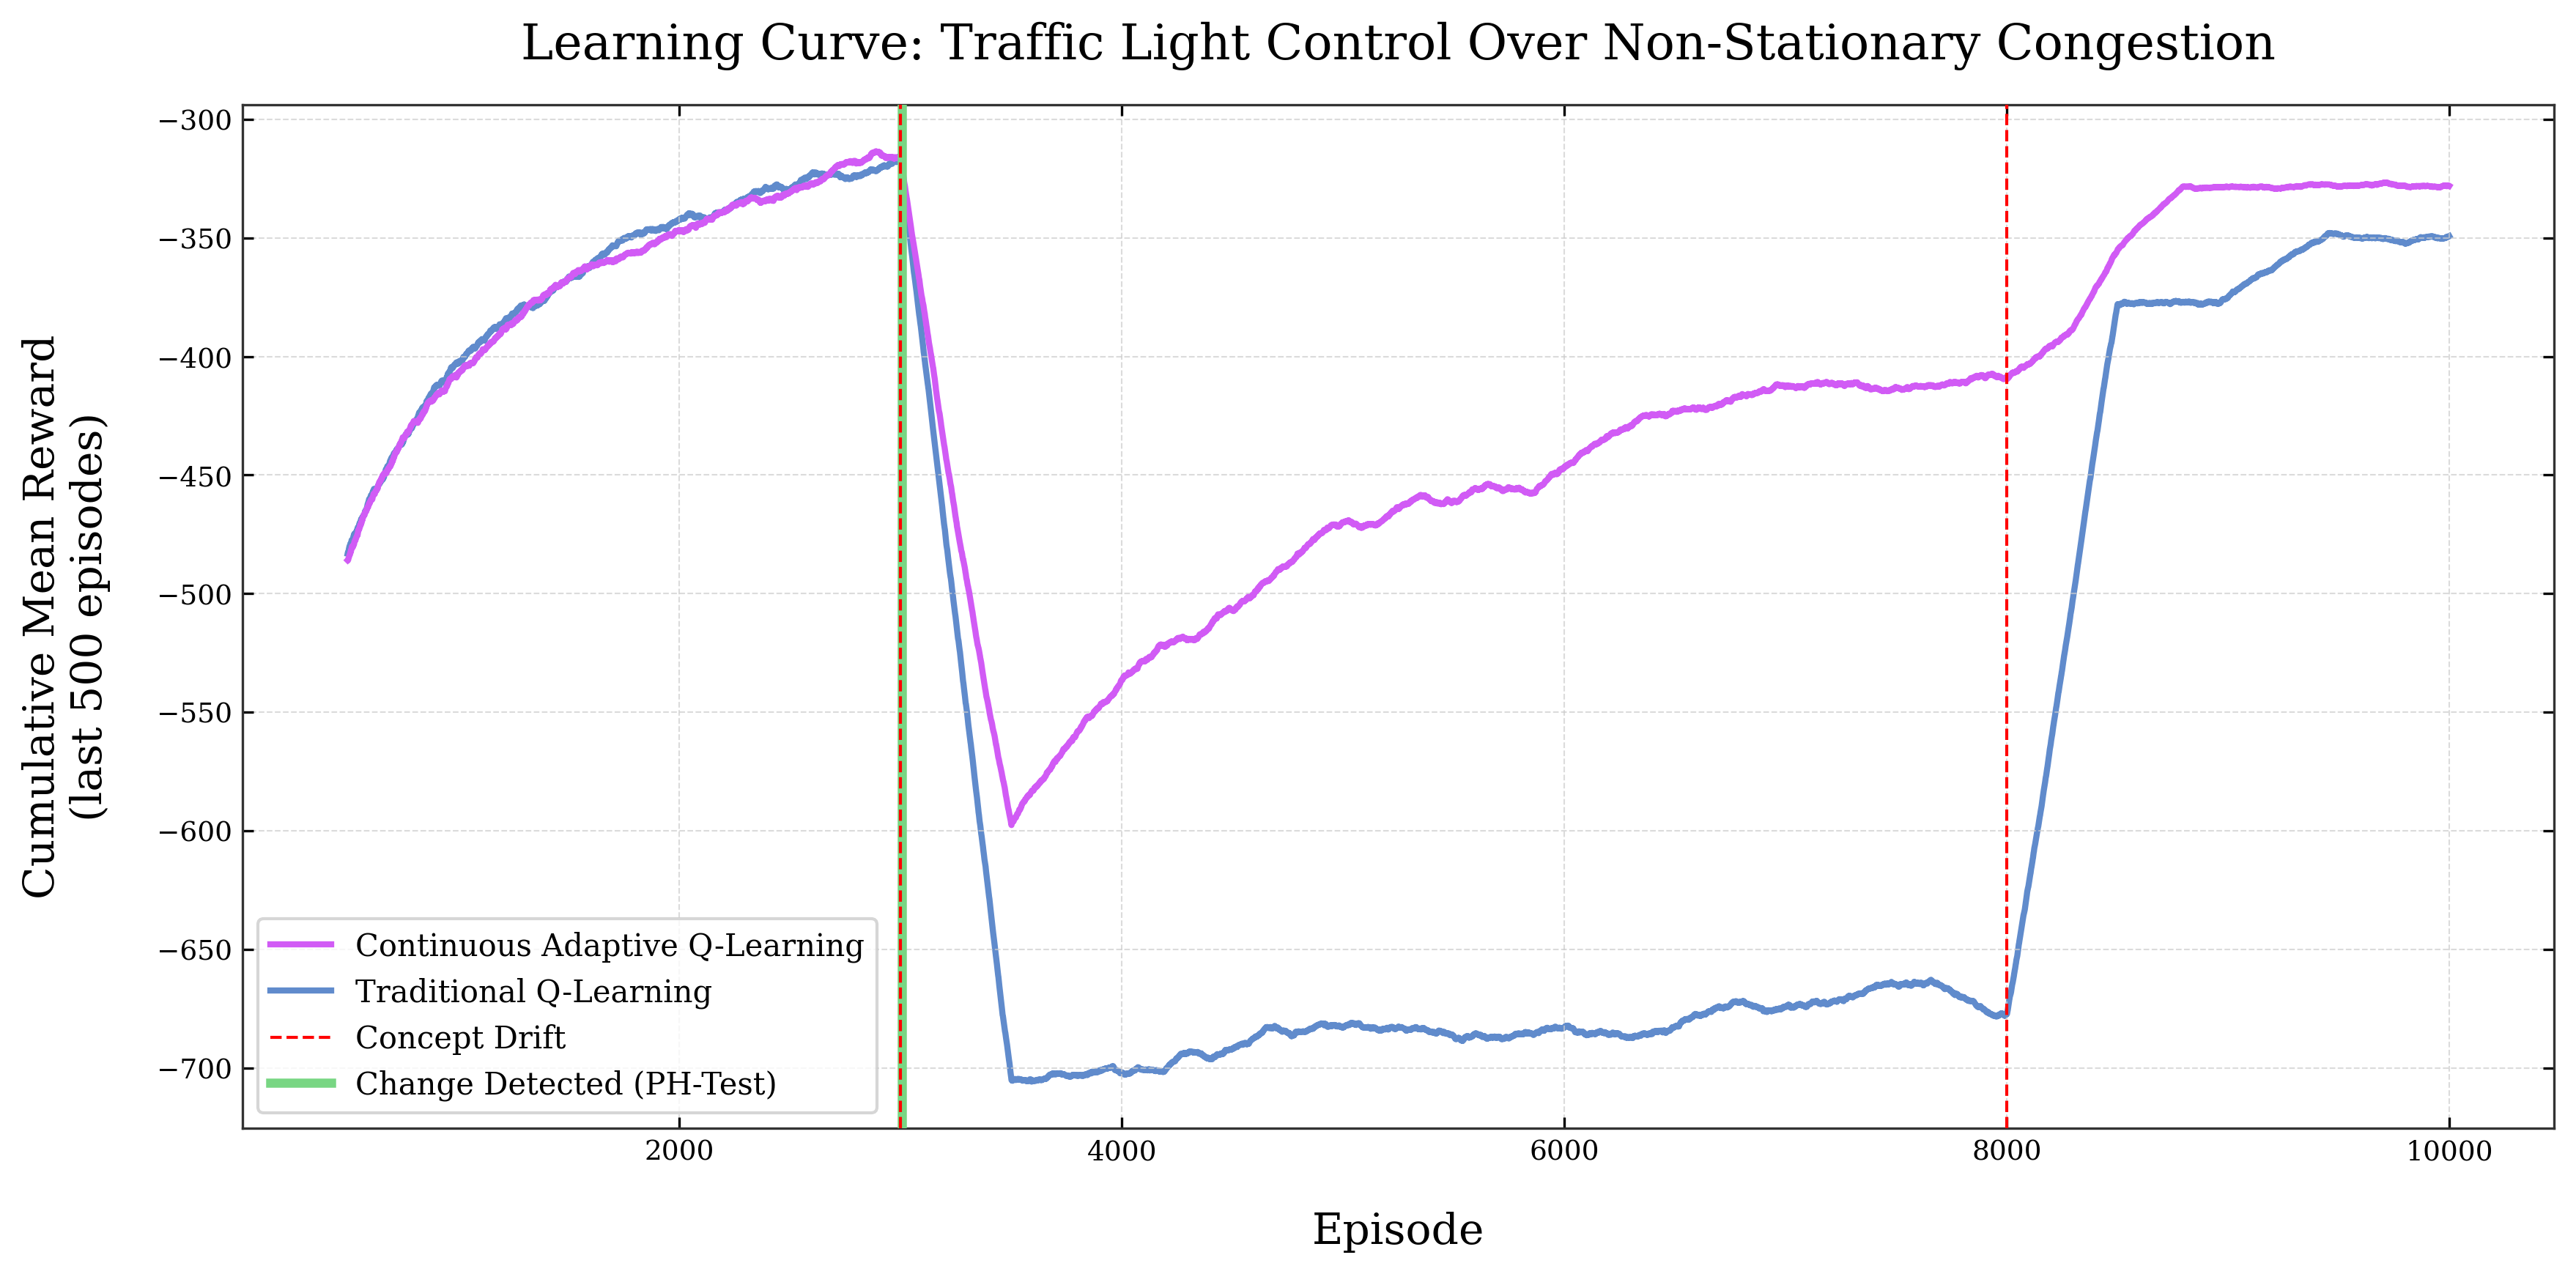
\includegraphics[width=0.9\textwidth]{figures/traffic_learning_curve}
    \caption{Learning performance for traffic-signal control under non-stationary congestion. \adaptiverl rapidly recovers after the first drift thanks to extension of action set after PH-Test detection, while traditional Q-learning suffers prolonged underperformance until the initial distribution is restored.}
    \label{fig:traffic-learning-curve}
\end{figure*}

In \fref{fig:traffic-learning-curve} we observe that after the first concept drift, \adaptiverl promptly 
increases exploration, and incorporates its new actions $(7,3)$ and $(3,7)$ in the agent's policy within 
a couple hundred episodes. With the new actions, performance starts to build up, effectively 
managing the new traffic conditions. In contrast, the baseline Q-learning agent demonstrate a deep 
performance loss, with only a slight performance gain over time. When the second concept drift 
occurs, restoring the traffic balance, both agents present a rapid performance improvement, as they 
are able to quickly exploit the initial policy. 

Finally, we observe the built-in penalty for wasted green time ensures \adaptiverl does not over-serve 
one lane as queues reduce, automatically balancing old and new phases without discarding any 
actions.

This traffic-signal control case study confirms that \adaptiverl can effectively:
\begin{enumerate}
  \item Detect and react to non-stationary conditions via the PH-test, boosting exploration as needed 
  and exploiting previous knowledge whenever possible; making for adaptable agents.
  \item Seamlessly incorporate new signal phases, analogous to real-world reprogramming of traffic 
  lights, without removing prior actions.
  \item Leverage a dynamic reward (with penalization) to avoid excessive servicing when traffic is light, 
  resulting in resource-efficient policies.
\end{enumerate}

This enables traffic controllers to update phase timings in real time, i.e., to be self-adaptive, 
 as \adaptiverl allows continuous automated adjustment to changing 
traffic patterns without manual retuning or agent retraining.


\endinput

